\section{Sphinx Packet Format}
\label{sec:sphinx}

HOPR uses the Sphinx packet format \cite{sphinxpaper} to encapsulate and route data packets in order to ensure sender and recipient unlinkability. The Sphinx packet format determines how mixnet packets are created and transformed before relaying them to the next downstream node in a way that does not leak path information to relayers or other parties. Each Sphinx packet consists of two parts, a header and an onion-encrypted payload:

\begin{figure}[H]
    \centering
    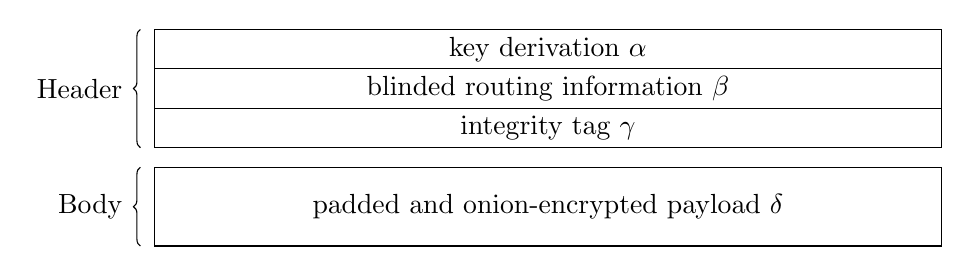
\begin{tikzpicture}
        \draw (0,0) rectangle (10,0.5);
        \draw (0,-0.5) rectangle (10,0);
        \draw (0,-1) rectangle (10,-0.5);

        \draw (5,0.25) node {key derivation $\alpha$};
        \draw (5,-0.25) node {blinded routing information $\beta$};
        \draw (5,-0.75) node {integrity tag $\gamma$};

        \draw[decoration={brace,raise=5pt,mirror},decorate] (0,0.5) -- node[left=8pt] {Header} (0,-1);

        \draw (0,-2.25) rectangle (10, -1.25);
        \draw (5,-1.75) node {padded and onion-encrypted payload  $\delta$};

        \draw[decoration={brace,raise=5pt,mirror},decorate] (0,-1.25) -- node[left=8pt] {Body} (0,-2.25);
    \end{tikzpicture}
    \label{fig:sphinxoverview}
    \caption{Schematic overview of a SPHINX packet}
\end{figure}

\subsection{Construction}

The following explains the steps a Sphinx packet goes through before arriving at its final destination. We start with key derivation to extract shared keys for the relay nodes chosen by the sender. These shared keys will be used to unblind the routing information and find the public key of the next relay node.

The integrity of this routing information is checked before sending. At each hop along the route, the relaying node replaces the routing information with their own blinding and decrypts one layer of the payload. Similar to onion routing, the payload has several layers of encryption, chosen such that the final layer is removed as the packet reaches its destination. However, as layers of encryption are removed, the packet is padded to keep the message length constant. This ensures that an adversary cannot draw any conclusions from message length about a transmission's position along the route.

\paragraph{Notation:}Let $\kappa=128$ be the security parameter. With non-negligible probability, an adversary must perform around $2^\kappa$ operations to break the security of Sphinx.

Let $r$ be the maximum number of nodes that a Sphinx mix message will traverse before being delivered to its destination.

$G$ is a prime order cyclic group satisfying the decisional Diffie-Hellman assumption \cite{Boneh_1998}. We use the secp256k1 elliptic curve \cite{secp}. The element $g$ is a generator of $G$ and $q$ is the (prime) order of $G$, with $q\approx2^{2*\kappa}$.

$G^*$ is the set of non-identity elements of G. $h_b$ is a pre-image resistant hash function used to compute blinding factors and modelled as a random oracle such that
$h_b:G^*\times G^*\rightarrow\mathbb{Z}^*_q$, where $\mathbb{Z}^*_q$ is the field of non-identity elements of $\mathbb{Z}_q$ (field of integers). We use the BLAKE2s hash function \cite{blake2}.

Each node $i$ has a private key $x_{i}\in \mathbb{Z}^*_q$ and a public key $y_{i}=g^{x_{i}}\in G^*$.
$\alpha_i$ is the group elements which, when combined with the nodes’ public keys, allow a shared key to be computed for each via Diffie-Hellman (DH) key exchange. This ensures that each node in the user-chosen route can forward the packet to the next, and only the receiving mix node can decrypt it.
$\varphi_i$ are the DH shared secrets, $b_i$ are the blinding factors.

\subsubsection{Key derivation}
\label{sec:sphinx:keyderivation}
The sender $A$ picks a random $x\in \mathbb{Z}^*_q$ that is used to derive new keys for every packet.

$A$ randomly picks a path consisting of intermediate nodes $B$, $C$, $D$, and the packet's final destination, $Z$.

$A$ performs an offline DH key exchange with each of these nodes and derives shared keys with each of them.

$A$ computes a sequence of $r$ tuples (in our case $r$=4)  $$(\alpha_0,\varphi_0,b_0),.................,(\alpha_{r-1},\varphi_{r-1},b_{r-1})$$ as follows:
$$\alpha_0=g^x,\varphi_0=y^x_B,b_0=h_b(a_0,\varphi_0)$$
and
\begin{equation}
    \begin{cases}
        \alpha_i=g^{x\Pi_{j=0}^{j=i-2}b_j}  \\
        \varphi_i=y^{x\Pi_{j=0}^{j=i-2}b_j} \\
        b_i=h_b(a_i,\varphi_i)
    \end{cases}\,.
    \label{eq:1}
\end{equation}
for $1\le i < r-1$, where $y_0,y_1, y_2, y_3$, and $y_4$ are the public keys of the nodes $B$, $C$, $D$, and $Z$, which we assume to be available to $A$ .
\subsubsection{Routing information}
Each node on the path needs to know which is the next downstream node. Therefore, the sender $A$ generates routing information $\beta_i$ for $B$, $C$, and $D$, as well as a message $END$ to tell $Z$ that it is the final recipient of the message. Whilst the keys for $B$, $C$, and $D$ are given as a compressed elliptic, the $END$ message occurs as a distinguished prefix.

In general, compression of elliptic curve points given as $(x,y)$ happens by taking the $x$-coordinate and the sign of $y$. If $y$ is above the $x$-axis, \texttt{0x02} is added, otherwise \texttt{0x03} is used. The $END$ message is given by \texttt{0x04} and is therefore easily distinguishable from public keys.

\begin{comment}
The $END$ message is a distinguished prefix byte which is added to the final recipient's compressed public key. For ECDSA public key compression, only the $x$ coordinate is used and is prepended by $02$.

The $y$ coordinate is extracted from $x$ by resolving the secp256k1 elliptic curve equation $Y^2=X^3+7$ \cite{secp}. A square root extraction will yield $Y$ or $-Y$. The compressed point format includes the least significant bit of $Y$ in the first byte (the first byte is $0\times02$ or $0\times03$, depending on that bit).
\end{comment}

The routing information is computed as follows:

\begin{align}
    \beta_{v-1} & =(y_Z\|0_{(2(r-v)+2)\kappa-|y_Z|}\oplus \rho(h_{\rho}(s_{v-1}))_{[ \,0....(2(r-v)+3)\kappa-1\,]})\|\phi_{v-1}                \\
    \text{and}  & \nonumber                                                                                                                    \\
    \beta_i     & =y_{i+1}\|\gamma_{i+1}\|\beta_{{i+1}_{[ \,0....(2r-1)\kappa-1\,] }}\oplus \rho(h_{\rho}(s_{i}))_{[ \,0....(2r+1)\kappa-1\,]}
    \label{eq:2}
\end{align}
$0\le i < v-1$

\begin{figure}[H]
    \centering
    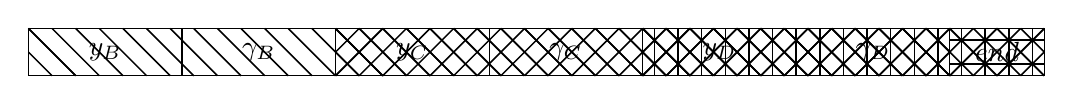
\begin{tikzpicture}
        \def\one{0.6}
        \def\scale{0.9}
        \def\nodeWidth{1.95}
        \def\endWidth{1.2}
        \def\width{3*2*\nodeWidth+\endWidth}
        \foreach \i\name in{0/B,1/C,2/D,3/Z} {
                \begin{scope}[shift={(\i*\nodeWidth*2,0)}]
                    \ifnum\i=0
                        \def\a{11.7}
                        \def\diff{11.1}
                    \fi

                    \ifnum\i=1
                        \def\a{7.8}
                        \def\diff{7.2}
                    \fi

                    \ifnum\i=2
                        \def\a{3.9}
                        \def\diff{3.3}

                    \fi

                    \ifnum\i=3
                        \def\a{\endWidth}
                        \def\diff{0.6}
                    \fi


                    \def\b{0.6}
                    \def\lw{0.2}

                    \foreach \x [count=\i] in{0,0.3,0.6,...,\b}{
                            \draw [line width=\lw mm](\x,0)--(0,\x) (\a-\b+\x,\b)--(\a,\x);
                        }
                    \foreach \x [count=\i] in{0,0.3,0.6,...,\diff}{
                            \draw [line width=\lw mm](\x+\b,0)--(\x,\b);
                        }

                    \ifnum\i>0
                        \foreach \x [count=\i] in{0,0.3,0.6,...,\b}{
                                \draw [line width=\lw mm](0,\x)--(\b-\x,\b) (\a-\b+\x,0)--(\a,\b-\x);
                            }
                        \foreach \x [count=\i] in{0,0.3,0.6,...,\diff}{
                                \draw [line width=\lw mm](\x,0)--(\b+\x,\b);
                            }
                    \fi

                    \ifnum\i>1
                        \foreach \x [count=\i] in{0.15,0.45,...,\a}{
                                \draw [line width=\lw mm](\x,0)--(\x,\b);
                            }
                    \fi

                    \ifnum\i>2
                        \foreach \x [count=\i] in{0.15,0.45,...,\b}{
                                \draw [line width=\lw mm](0,\x)--(\a,\x);
                            }
                    \fi
                \end{scope}
                \ifnum\i<3
                    \draw [color=white] (\i*2*\nodeWidth,0) rectangle (\i*2*\nodeWidth+\nodeWidth,\one) node [midway,color=black] {$y_{\name}$};
                    \draw (\i*2*\nodeWidth,0) -- (\i*2*\nodeWidth,\one);
                    \draw [color=white] (\i*2*\nodeWidth+\nodeWidth,0) rectangle (\i*2*\nodeWidth+2*\nodeWidth,\one) node [midway,color=black] {$\gamma_{\name}$};
                    \draw (\i*2*\nodeWidth+\nodeWidth,0) -- (\i*2*\nodeWidth+\nodeWidth,\one);
                \else
                    \draw [color=white] (\i*2*\nodeWidth,0) rectangle (\i*2*\nodeWidth+\endWidth,\one) node [midway,color=black] {$end$};
                    \draw (\i*2*\nodeWidth,0) -- (\i*2*\nodeWidth,\one);
                \fi
            }

        \draw (0,0) rectangle (\width,\one);
    \end{tikzpicture}
    \caption{Routing information}
\end{figure}

such that $y_Z$ is the destination's public key in compressed form (since this is only the $x$-coordinate, it is 33 bytes instead of 64) and $|y_Z|$ is its length. $\rho$ is a pseudorandom generator (PRG) and $h_{\rho}$ is the hash function used to key $\rho$.
$v\leq r$ is the length of the path traversed by the packet, where $|y_Z| \leq (2(r - v) + 2)$. $\phi$ is a filler string such that
\begin{align}
    \phi_i & =\{ \phi_{i-1}\|0_{2\kappa}\}\oplus \rho(h_{\rho}(s_{i-1}))_{[ \,(2(r-i)+3)\kappa..(2r+3)\kappa-1\,]}
\end{align}
where $\phi_0=\epsilon$ is an empty string. $\phi_i$ is generated using the shared secret $s_{i-1}$ and used to ensure the header packets remain constant in size as layers of encryption are added or removed. Upon receiving a packet, the processing node extracts the information destined for it from the route information and the per-hop payload. The extraction is performed by deobfuscating and left-shifting the field. Ordinarily, this would make the field shorter at each hop, allowing an attacker to deduce the route length. For this reason, the field is pre-padded before forwarding. Since the padding is part of the HMAC, the origin node will have to pre-generate an identical padding (to that generated at each hop) in order to compute the HMACs correctly for each hop.

$\beta_i$ is computed as the concatenation of $y_Z$ and a sequence of padding which is then encrypted by XORing with the output of a PRG seeded with shared key $s_{v-1}$ of node $v-1$. The result is finally concatenated with $\phi$ to ensure the header packets remain constant in size.

In the original Sphinx paper, $y_Z$ is concatenated with an identifier $I$ and $0$ padding sequence, where $I$ is used for SURBs (single-use reply blocks) such that $I \in \{0, 1\}^\kappa$. We do not use $I$ since HOPR does not currently employ SURBs. We do, however, include $hint$ and $challenge$ values in $\beta$, defined in the \lcnameref{sec:proofofrelay} section. These values are not included in the original Sphinx paper but are needed for the HOPR protocol. Since $A$ has a shared secret with each of the nodes along the path, it is able to derive blindings for each of them. Each node along the path receives an authentication tag $\gamma_i$ in the form of a message authentication code (MAC), which is encoded in the header.

Padding is added at each mix stage in order to keep the length of the message invariant at each hop.

The mix header is constructed as follows:
\begin{align}
    M_i & =(\alpha_i,\beta_i,\gamma_i)
\end{align}

$A$ sends the mix header $M_0$ to $B$. Once $B$ receives the packet, it derives the shared key $s_0$ by computing

$$s_0=(\alpha_0)^b=(g^x)^b=(g^b)^x=y^x_B$$

and removes its blindings. Here $b$ is the private key of node B. This allows $B$ to unblind the routing info that tells $B$ the public key of the next downstream node, $C$. The process happens in the same fashion for all further downstream nodes after $B$.


\subsubsection{Integrity check}
The integrity check allows the node to verify whether or not the header has been modified. By using the derived shared secret $\varphi_i$, each node is able to recompute the authentication tag and check the integrity of the received packet as follows:
\begin{align}
    \gamma_i & =HMAC(s_i,\beta_i)
    \label{eq:6}
\end{align}
$B$ computes the keyed hash of the encrypted routing information $\beta_0$ as

$$\gamma_0=HMAC(s_0,\beta_0)$$
and compares with the integrity tag $\gamma_0$ attached in the packet header. If the integrity check fails, it is assumed the header has been tampered with and the packet is dropped. Otherwise, the mix node proceeds to the unblinding step. The HOPR packet header contains one integrity tag $\gamma_i$ for each node along the path.
\subsubsection{Unblinding}
\label{sec:sphinx:unblinding}

The unblinding works as follows: $B$ decrypts the attached $\beta_0$ in order to extract the routing instructions. First, $B$ appends a zero-byte padding at the end of $\beta_0$ and decrypts the padded block of routing information $\beta$ by XORing it with $PRG(s_{0})$ as follows:
\begin{align}
    (\beta_0\|0_{2\kappa}) & \oplus \rho(h_{\rho}(s_{0}))
\end{align}
$B$ parses the routing instructions from $A$ in order to obtain the address of the next mix node, $C$, as well the new integrity tags $\gamma_1$ and $\beta_1$, which should be forwarded to the next hop.
\subsubsection{Delete and shift}
After $B$ extracts the public key of $C$, it deletes the routing information from the packet. $B$ then fills the empty space with its own blinding (which is different from the one received from $A$) by setting the key share $\alpha_0$ to $\alpha_1=g^{xb_0}$. $B$ also computes $\beta_1$ as follows:

The first $\kappa$ bits of $\beta_0$ will be $n_{1}$ itself, the next $\kappa$ bits will be $\gamma_{1}$, and the remaining $(2r-1)\kappa$ bits of $\beta_0$ are shifted left to form the leftmost $(2r-1)\kappa$ bits of $\beta_{1}$; the rightmost $2\kappa$ bits of $\beta_{1}$ are simply a substring of an output of the PRG function.

\begin{figure}[H]
    \centering
    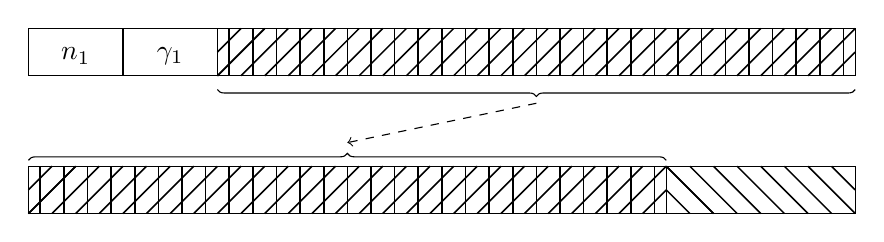
\begin{tikzpicture}
        \def\betaLength{10.5}
        \def\pubKey{1.2}
        \def\authTag{1.2}
        \draw (0,0) rectangle (\betaLength,0.6);

        \draw (0.6, 0.25) node {$n_1$};
        \draw (1.8, 0.25) node {$\gamma_1$};

        \draw (\pubKey,0) -- (\pubKey,0.6) (\pubKey+\authTag,0) -- (\pubKey+\authTag,0.6);

        \draw[decoration={brace,raise=5pt,mirror},decorate] (\authTag+\pubKey,0) -- (\betaLength,0);

        \def\halfBeta{{(\betaLength-\pubKey-\authTag)}*0.5}
        \draw [->,dashed] (4.05+\pubKey+\authTag, -0.35) -- (4.05, -0.85);

        \draw[decoration={brace,raise=5pt},decorate] (0,-1.25) -- (\betaLength-\authTag-\pubKey,-1.25);

        \begin{scope}[shift={(\pubKey+\authTag,0)}]
            \def\a{8.1}
            \def\b{0.6}
            \def\lw{0.2}
            \def\diff{7.5}

            \foreach \x [count=\i] in{0,0.3,0.6,...,\b}{
                    \draw [line width=\lw mm](0,\x)--(\b-\x,\b) (\a-\b+\x,0)--(\a,\b-\x);
                }
            \foreach \x [count=\i] in{0,0.3,0.6,...,\diff}{
                    \draw [line width=\lw mm](\x,0)--(\b+\x,\b);
                }

            \foreach \x [count=\i] in{0,0.15,0.45,...,\a}{
                    \draw [line width=\lw mm](\x,0)--(\x,\b);
                }
        \end{scope}

        \begin{scope}[shift={(0, -1.75)}]
            \draw (0,0) rectangle (\betaLength,0.6);
            \draw (\betaLength-\pubKey-\authTag, 0) -- (\betaLength-\pubKey-\authTag, 0.6);

            \begin{scope}[shift={(0,0)}]
                \def\a{8.1}
                \def\b{0.6}
                \def\lw{0.2}
                \def\diff{7.5}

                \foreach \x [count=\i] in{0,0.3,0.6,...,\b}{
                        \draw [line width=\lw mm](0,\x)--(\b-\x,\b) (\a-\b+\x,0)--(\a,\b-\x);
                    }
                \foreach \x [count=\i] in{0,0.3,0.6,...,\diff}{
                        \draw [line width=\lw mm](\x,0)--(\b+\x,\b);
                    }

                \foreach \x [count=\i] in{0,0.15,0.45,...,\a}{
                        \draw [line width=\lw mm](\x,0)--(\x,\b);
                    }
            \end{scope}

            \begin{scope}[shift={(\betaLength-\pubKey-\authTag,0)}]
                \def\a{2.4}
                \def\b{0.6}
                \def\lw{0.2}
                \def\diff{1.8}
                \foreach \x [count=\i] in{0,0.3,0.6,...,\b}{
                        \draw [line width=\lw mm](\x,0)--(0,\x) (\a-\b+\x,\b)--(\a,\x);
                    }
                \foreach \x [count=\i] in{0,0.3,0.6,...,\diff}{
                        \draw [line width=\lw mm](\x+\b,0)--(\x,\b);
                    }
            \end{scope}
        \end{scope}

    \end{tikzpicture}
    \caption{Shifting in the header}
\end{figure}

The new mix header is now ready to be sent to $C$, defined as the node with public key $y_1$:

$$M_1=(\alpha_1,\beta_1,\gamma_1)$$

where $\alpha$, $\beta$ and $\gamma$ are defined in equations $\ref{eq:1}$, $\ref{eq:2}$ and $\ref{eq:6}$
\subsubsection{Encrypt and decrypt}

In contrast to the header, the integrity of the payload is not directly protected by the protocol. To make potential manipulations of the message nonetheless visible to the final recipient of the message, hiding the content of the payload is done using a pseudorandom permutation scheme (PRP) and its inverse to undo the transformation. This comes with the property that if there were any modifications to the payload such as a bit flip, the probability that the decoded message contains any relevant information is expected to be negligible.

To implement the PRP, HOPR makes use of the LIONESS \cite{lionesspaper} wide-block cipher scheme, instantiated by using Chacha20 as a stream cipher and BLAKE2s as a hash function as suggested by \href{https://katzenpost.mixnetworks.org/docs/specs/lioness.html}{Katzenpost}, see appendix \ref{appendix:lioness} for a detailed description and the chosen parameters.

During creation of the packet, the sender derives, as seen in section \ref{sec:sphinx:keyderivation}, a shared key $s_i$ with each node along the chosen path and uses them to create subkeys $s_i^{prp}$ to key the PRP. See Appendix \ref{appendix:keyderivation} for more details about the key derivation.

To provide the final recipient the opportunity to determine whether a message \textit{is} meaningful content or not, each message is padded by a protocol-specific tag $\tau$ and 0s to fit the packet size of 500 bytes, yielding $m_{pad}$. Decoded payloads that do not include $\tau$ are considered invalid and should be dropped.

\begin{figure}[H]
    \centering
    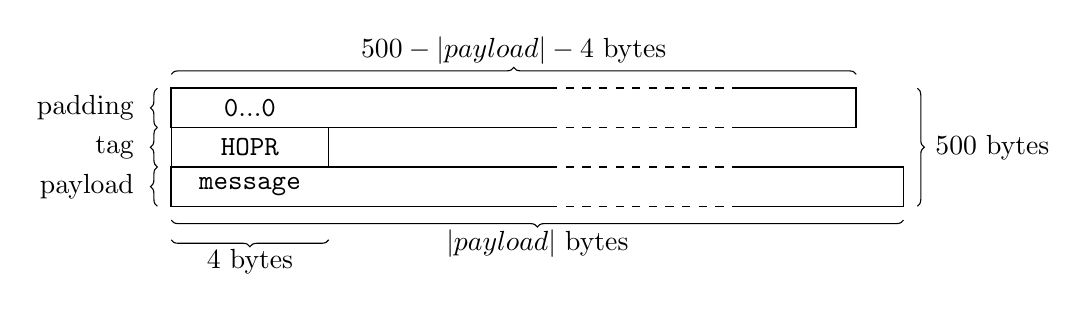
\begin{tikzpicture}
        \def\one{0.3}
        \def\lw{0.2}
        \def\middle{16*\one}
        \def\offset{8*\one}
        \def\packetLength{500}

        \def\paddingLength{29*\one}
        \def\payloadLength{31*\one}


        \draw[decoration={brace,raise=5pt},decorate] (0,0.5) -- node[above=5pt] {$\packetLength - |payload| - 4$ bytes} (\paddingLength,0.5);
        \begin{scope}
            \draw[decoration={brace,raise=5pt},decorate] (0,0) -- node[left=10pt] {padding} (0,0.5);
            \def\width{\paddingLength}
            \draw (1,0.25) node {$\mathtt{0...0}$};
            \draw [line width=\lw mm] (\middle,0.5) -- (0,0.5) --  (0,0) -- (\middle,0);
            \draw [line width=\lw mm] (\middle,0) --  (\middle+\offset, 0) [dashed];
            \draw [line width=\lw mm] (\middle,0.5) --  (\middle+\offset, 0.5) [dashed];
            \draw [line width=\lw mm] (\middle+\offset,0.5) -- (\width,0.5) --  (\width,0) -- (\middle+\offset,0);
        \end{scope}

        \begin{scope}[shift={(0,-0.5)}]
            \draw[decoration={brace,raise=5pt},decorate] (0,0) -- node[left=10pt] {tag} (0,0.5);
            \draw [draw] (0,0) rectangle (2,0.5);
            \draw (1,0.25) node {$\mathtt{HOPR}$};
        \end{scope}

        \begin{scope}[shift={(0,-1)}]
            \draw[decoration={brace,raise=5pt},decorate] (0,0) -- node[left=10pt] {payload} (0,0.5);
            \draw (1,0.25) node {$\mathtt{message}$};
            \def\width{\payloadLength}
            \draw [line width=\lw mm] (\middle,0.5) -- (0,0.5) --  (0,0) -- (\middle,0);
            \draw [line width=\lw mm] (\middle,0) --  (\middle+\offset, 0) [dashed];
            \draw [line width=\lw mm] (\middle,0.5) --  (\middle+\offset, 0.5) [dashed];
            \draw [line width=\lw mm] (\middle+\offset,0.5) -- (\width,0.5) --  (\width,0) -- (\middle+\offset,0);
        \end{scope}

        \draw[decoration={brace,raise=5pt,mirror},decorate] (0,-1.0) -- node[below=5pt] {$|payload|$ bytes} (\payloadLength,-1.0);
        \draw[decoration={brace,raise=5pt,mirror},decorate] (0,-1.25) -- node[below=5pt] {4 bytes} (2,-1.25);

        \draw[decoration={brace,raise=5pt},decorate] (\payloadLength,0.5) -- node[right=8pt] {$\packetLength$ bytes} (\payloadLength,-1.0);
    \end{tikzpicture}
    \caption{Padded message consisting of 0-padding, protocol tag $\tau$ ($\mathtt{0x484f5052}$, ASCII-encoded ``HOPR"), and payload $m$.}
\end{figure}

The sender takes the padded message and encrypts it using $\mathsf{PRP.permutate}$ with the derived subkeys in reverse order ($...,s_{i+1}^{prp}, s_i^{prp}, s_{i-1}^{prp},....$) $$\delta_i = \mathsf{PRP.permutate}_{s_i^{prp}}(\delta_{i+1})$$ where $\delta_4 = m_{pad}$ and $\delta_0$ is the ciphertext that is sent to the first relayer when using three intermediate hops.

Each node $n_i$ along the chosen path then removes one layer of encryption by setting $$\delta_{i-1} = \mathsf{PRP.inverse}_{s_i^{prp}}(\delta_i)$$ yielding $\delta_0 = m_{pad}$ in case the node is the final recipient.



\subsection{Implementation choices}

HOPR employs the following cryptographic primitives:

\begin{itemize}
    \item \textbf{Cyclic group} HOPR's Sphinx implementation uses an elliptic curve group on the secp256k1 curve. Operations are therefore performed on the elliptic curve.

    \item \textbf{Hash function} HOPR uses the BLAKE2s hash function, a cryptographic hash function faster than SHA-2 and SHA-3, yet at least as secure as SHA-3. It produces digests of 32 bytes.

    \item \textbf{MAC} HOPR uses HMAC based on the BLAKE2s hash function.

    \item \textbf{Encryption scheme} HOPR uses the LIONESS \cite{lionesspaper} implementation, using BLAKE2s as a hash function and ChaCha20 as a stream cipher.

    \item \textbf{Padding} The original Sphinx paper uses a sequence of 0s for padding. However, this allows the last mix node in the path to infer information about the length of the path and the last destination, hence breaking one of the security properties promised by Sphinx. In order to prevent this attack, HOPR replaces the 0-padding with randomized padding for the last exit-mix node when $v<r$. This ensures the exit node cannot identify where the padding starts and thus will not be able to determine the path length. In the case where $v=r$ there is no need to add padding as the length of the path is the maximum length, and thus no additional information is being revealed.

\end{itemize}
